\section{Results \& Discussion}

% was erzähle ich hier?

\Cref{fig:timmean} illustrates the spatial distribution of mean precipitation: The general pattern of different grid resolutions is similar, depicting high precipitation rates over the Northern Atlantic and at the coasts of Iceland, Norway and Scotland. However, it is evident that using high grid resolution locally increases the intensity of precipitation.

\begin{figure}[h]
	\centering
	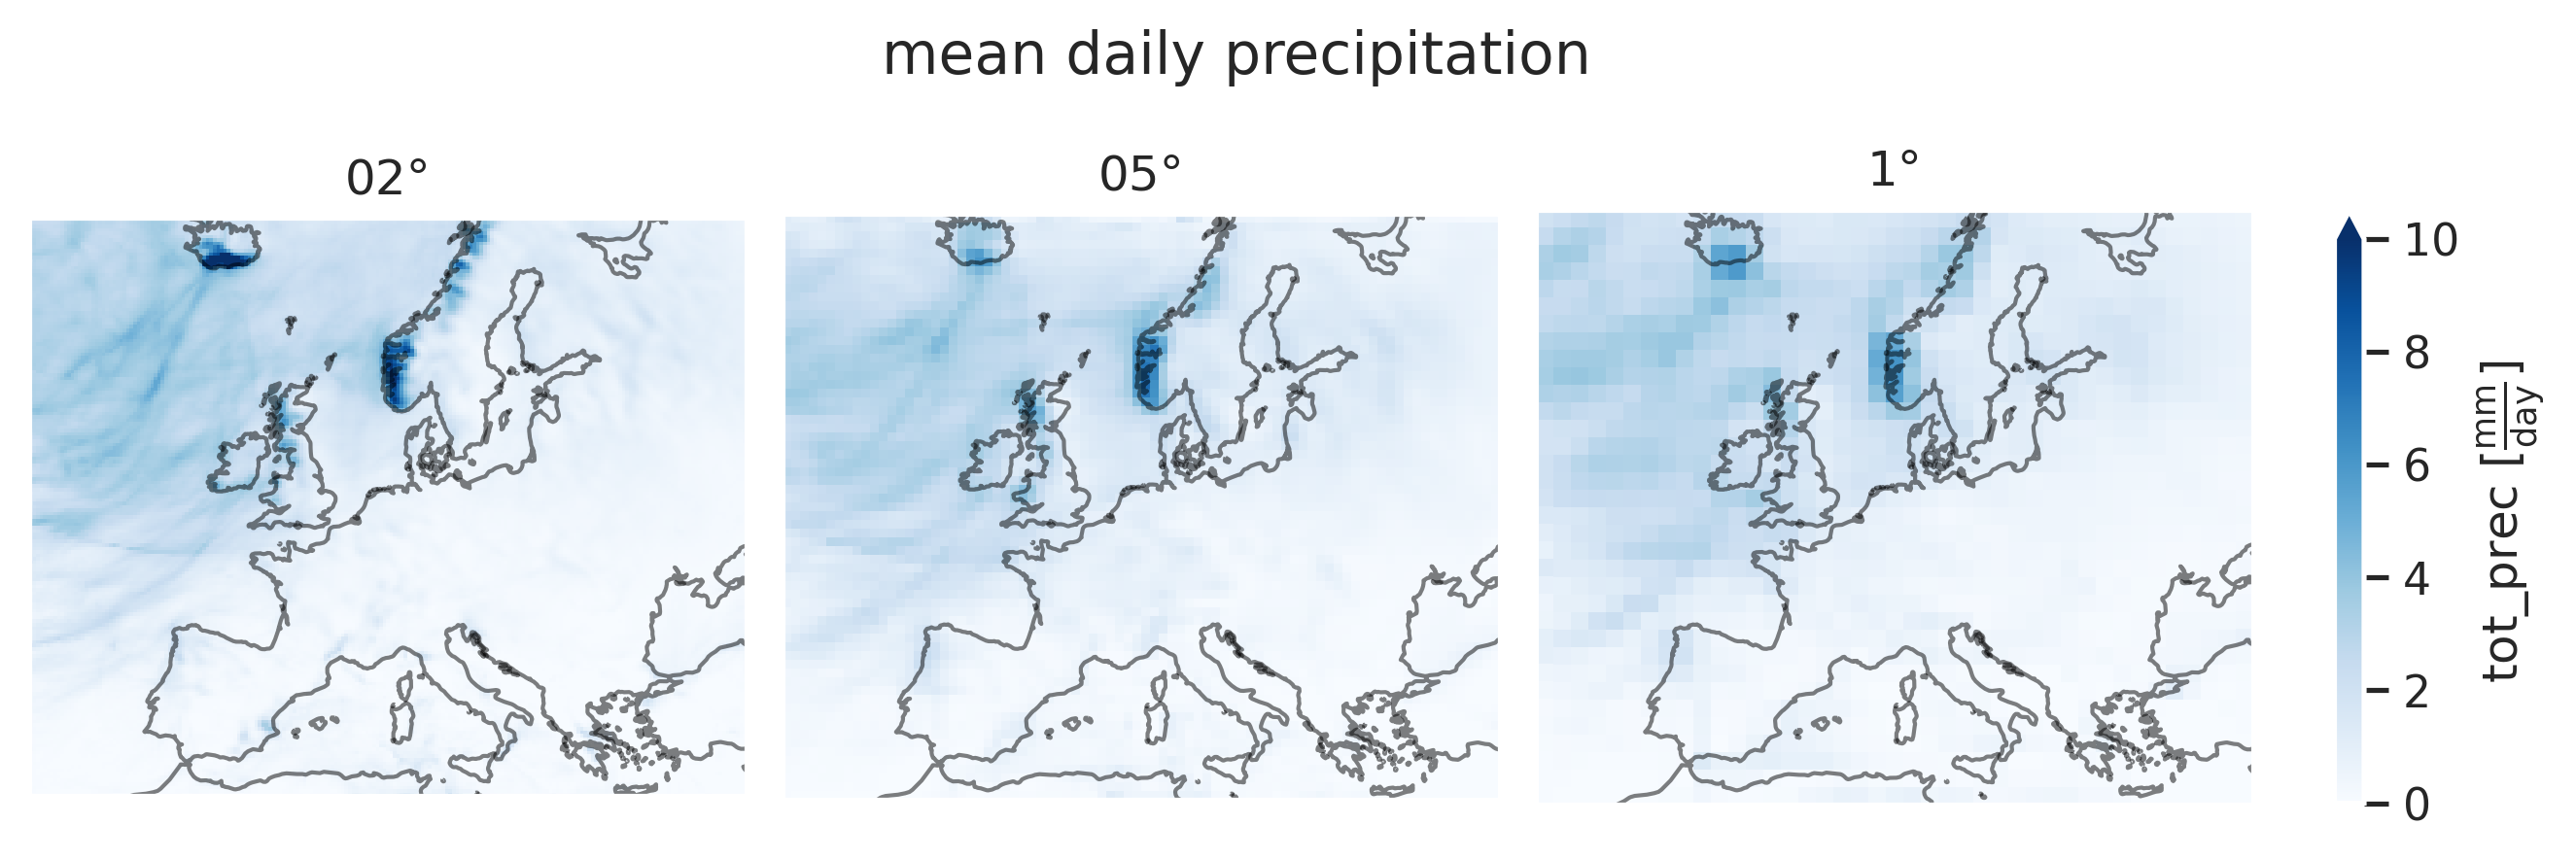
\includegraphics[width=\figwidth]{../figs/2-timmean.png}
	\caption{Temporal mean of daily precipitation sum throughout January 1990 for different grid resolutions.}
	\label{fig:timmean}
\end{figure}

\begin{figure}
	\centering
	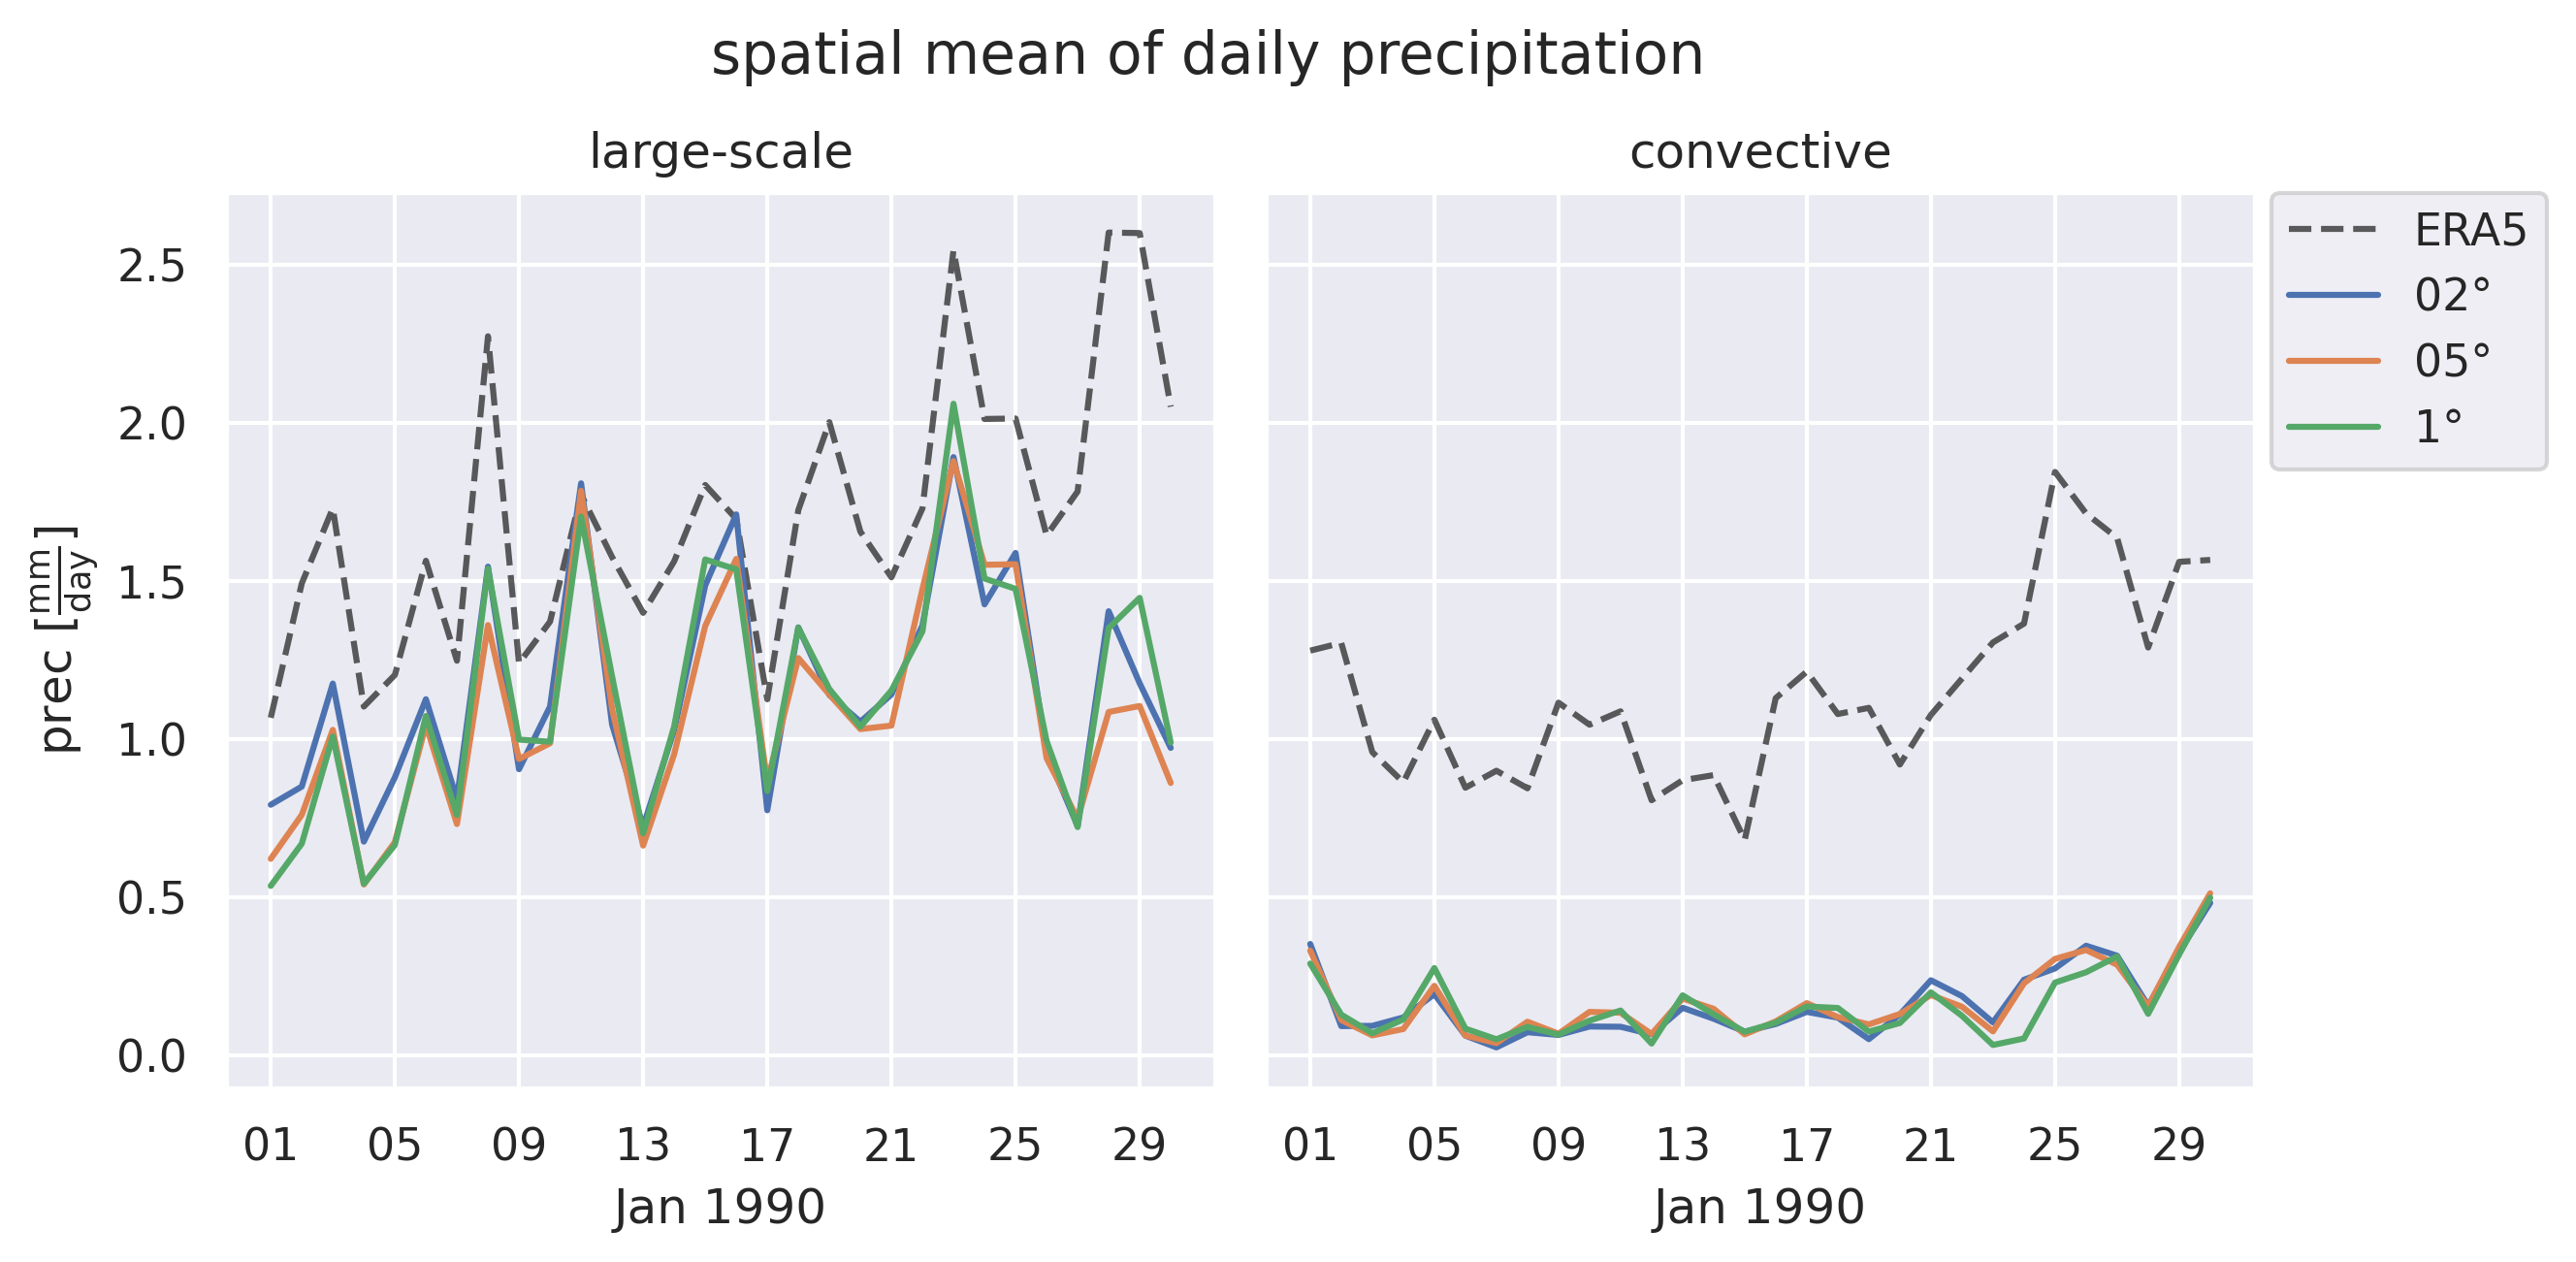
\includegraphics[width=\figwidth]{../figs/5-gsp-con.png}
	\caption{Spatial mean of daily precipitation sum split into large-scale (i.e., grid-scale) and convective signal for different grid resolutions. ERA5 reanalysis data as reference.}
	\label{fig:fldmean}
\end{figure}

When focussing on the temporal domain, the daily precipitation signals of the CCLM simulations are---generally speaking---similar, indicating that the daily sum over the entire (cropped) model region does not change considerably with model resolution. In \cref{fig:fldmean}, precipitation is split into a grid-scale and convective component, and ERA5 data is included as a reference.
In both subplots, simulations underestimate the observed daily precipitation sum, although the difference between reference and simulation is more pronounced for convective precipitation. The underlying trend in simulation and reference of grid-scale precipitation is comparable, which validates the model results on broader scales. It is important to note though that the simulations have been driven with ERA-Interim data and are now compared to ERA5 data, which might introduce additional biases triggered by different data assimilation procedures of the reanalyses.

The \textit{absolute} difference in precipitation between grid resolutions is more pronounced in the grid-scale precipitation, although without a consistent signal. E.g., in the beginning of January, 0.2°-resolution shows more grid-scale precipitation compared to the remaining resolutions, in the end of the month though, 0.2°- and 1°-resolution show a similar signal, while 0.5°-resolution simulates less grid-scale precipitation. In contrast, variation in the convective part is relatively small. The missing deep convection scheme might be the reason for this observation, since in such a case convective precipitation is derived from vertical turbulence only.

\begin{figure}
	\centering
	\includegraphics[width=\figwidth]{../figs/4-hovmöller.png}
	\caption{Hovmöller plot of the meridional mean of daily precipitation sum on the \(x\)-axis (units in \textit{rotated} longitude) and time domain in days on \(y\)-axis. CCLM simulations of different grid resolution and ERA5 reanalysis data displayed. Precipitation below \SI{0.5}{\mm\per\day} is excluded.}
	\label{fig:hovmöller}
\end{figure}

One way to combine information from the spatial and temporal domain is displayed in \cref{fig:hovmöller}. The Hovmöller diagram illustrates how precipitation events follow the dominant westerly flow of the Northern Hemisphere. On top, precipitation is more intense in the western part of the model region (as already indicated by \cref{fig:timmean}, especially over the Atlantic Ocean), and starts to decrease over the land masses of Northern and Central Europe. Again, simulated precipitation underestimates the reanalysis data in the entire model region. In particular, the presumingly convective events at \SIrange{-5}{0}{°} rotated longitude are not present in the simulations (apart from one in mid-January).
The high grid resolution has a strong localization of precipitation extremes, but tends to underestimate their spread. For example, in the end of January, the 0.2°-resolution shows small-scale structures of intense precipitation in the west, but fails to simulate the large area of moderate precipitation further in the east. The lower resolutions cannot reproduce the intensity of the strong events in the west, but the 1°-resolution shows zonal precipitation structures until far into the east, which match the pattern of the reanalysis data. For further details about this individual event refer to \cref{fig:app-event} in \cref{sec:app}.